%Standard stuff
  \documentclass[a4paper,10pt,english]{article}
  \usepackage[utf8]{inputenc}
  \usepackage[english]{babel}
  \usepackage{amsmath,graphicx,varioref,verbatim,amsfonts,geometry,enumerate,commath,textcomp,listings,siunitx,float}
  % colors in text
  \usepackage[usenames,dvipsnames,svgnames,table]{xcolor}
  % Hyper refs
  \usepackage[colorlinks]{hyperref}
  % inkspace
  \usepackage{import}
  \usepackage{xifthen}
  \usepackage{pdfpages}
  \usepackage{transparent}
  \usepackage{tikz,pgfplots,cancel}

%Biber
\usepackage[backend=biber, style=chicago-authordate]{biblatex}
  \AtEveryBibitem{%
    \clearlist{language}}

% Colour scheme for hyperlinks
  \hypersetup{%
    colorlinks,
    citecolor=Blue,
    linkcolor=Blue,
    urlcolor=Blue}

% Document formatting
  \setlength{\parindent}{0mm}
  \setlength{\parskip}{1.5mm}
  \definecolor{mygreen}{RGB}{28,172,0} % color values Red, Green, Blue
  \definecolor{mylilas}{RGB}{170,55,241}
% Color scheme for listings
  \usepackage{textcomp}
  \definecolor{codegreen}{rgb}{0,0.6,0}
  \definecolor{codegray}{rgb}{0.5,0.5,0.5}
  \definecolor{codepurple}{rgb}{0.58,0,0.82}
  \definecolor{backcolour}{rgb}{0.95,0.95,0.92}
  \definecolor{listinggray}{gray}{0.9}
  \definecolor{lbcolor}{rgb}{0.9,0.9,0.9}
  \lstdefinestyle{mystyle}{
    backgroundcolor=\color{backcolour},
    commentstyle=\color{codegreen},
    keywordstyle=\color{magenta},
    numberstyle=\tiny\color{codegray},
    stringstyle=\color{codepurple},
    basicstyle=\ttfamily\footnotesize,
    breakatwhitespace=false,
    breaklines=true,
    captionpos=b,
    keepspaces=true,
    numbers=left,
    numbersep=5pt,
    showspaces=false,
    showstringspaces=false,
    showtabs=false,
    tabsize=2
  }

  \lstset{style=mystyle}

%for toc
  \usepackage{tocloft}
  \addtolength{\cftsubsecnumwidth}{40pt}

% new commands
  \newcommand{\dd}[1]{\mathrm{d}#1}
  \def\doubleunderline#1{\underline{\underline{#1}}}
  \newcommand{\uvec}[1]{\boldsymbol{\hat{\textbf{#1}}}}
  \renewcommand{\thesection}{Problem \arabic{section}}

%ne pas modifier ou enlever la ligne ci-haut
% \documentclass[11pt,letterpaper]{article}

%2015-08-26 - Document préparé par David Lafrenière, pour le cours PHY1234.

%Pour langue et caractères spéciaux
% \usepackage[english]{babel}
% \usepackage[T1]{fontenc}
% \usepackage{lmodern}
% \usepackage[utf8]{inputenc}
% \usepackage{multicol}
% \usepackage{gensymb}
% \usepackage{MnSymbol}
% \usepackage{xcolor}
% \usepackage{soul}
% \usepackage{units}
% \usepackage{makecell}
% \usepackage{wasysym}
% \usepackage{subfig}
% \usepackage{listings}
% \usepackage{amsmath}
% \usepackage{physics}
% \usepackage[usenames,dvipsnames,svgnames,table]{xcolor}
% \usepackage[colorlinks]{hyperref}

% \definecolor{codegreen}{rgb}{0,0.6,0}
% \definecolor{codegray}{rgb}{0.5,0.5,0.5}
% \definecolor{codepurple}{rgb}{0.58,0,0.82}
% \definecolor{backcolour}{rgb}{0.95,0.95,0.92}

% %Biber
% \usepackage[backend=biber, style=chicago-authordate]{biblatex}
%   \AtEveryBibitem{%
%     \clearlist{language}}

% % Colour scheme for hyperlinks
%   \hypersetup{%
%     colorlinks,
%     citecolor=Blue,
%     linkcolor=Blue,
%     urlcolor=Blue}

% \lstdefinestyle{mystyle}{
%     backgroundcolor=\color{backcolour},
%     commentstyle=\color{codegreen},
%     keywordstyle=\color{magenta},
%     numberstyle=\tiny\color{codegray},
%     stringstyle=\color{codepurple},
%     basicstyle=\ttfamily\footnotesize,
%     breakatwhitespace=false,
%     breaklines=true,
%     captionpos=b,
%     keepspaces=true,
%     numbers=left,
%     numbersep=3pt,
%     showspaces=false,
%     showstringspaces=false,
%     showtabs=false,
%     tabsize=2
% }

% \lstset{style=mystyle}


% %Pour ajuster les marges
% %\usepackage[top=2cm, bottom=2cm, left=1.4cm, right=1.4cm, columnsep=20pt]{geometry}


% %pour inclure des graphiques
% \usepackage{graphicx}
% \usepackage{float}
% \usepackage{amsmath}

% %Pour inclure des adresse web
% \usepackage{url}

% %pour inclure les codes en annexe
% \usepackage{fancyvrb}
% \usepackage{listingsutf8}
% \usepackage{color}
% \lstset{inputencoding=utf8/latin1,numbers=left,numberstyle=\footnotesize,frame=single,commentstyle=\it\color{blue},keywordstyle=\bf\color{red}}

% \begin{document}

%Page titre
% \begin{titlepage}
% \center

% \vspace*{2cm}

% \textsc{\LARGE University of Oslo}\\[1cm]
% \textsc{\Large FYS4150-3150}\\[1.5cm]

% \rule{\linewidth}{0.5mm} \\[0.5cm]
% {\LARGE \bfseries Project 1} \\[0.2cm] % ***éditez ceci***
% \rule{\linewidth}{0.5mm} \\[5cm]

% \textbf{\Large  Martaillé Richard Eloi}\\
% %{\Large Student number : 669517}\\[8cm]
% \textbf{\Large  Vebjørn Øvereng}\\
% \textbf{\Large  Christophe Kristian Blomsen}\\
% \textbf{\Large  Vetle Henrik Hvoslef}\\
% % this was not very pretty

%\addbibresource{/home/chris/.refs/refs.org} % Entries are in the "refs.bib" file
  \author{Christophe Kristian Blomsen\\
    \texttt{c.k.blomsen@astro.uio.no}
    \and
    Eloi Richard Martaillé\\
    \texttt{e.m.richard@astro.uio.no}
    \and
    Vebjørn Øvereng\\
    \texttt{vebjoro@uio.no}
    \and
    Vetle Henrik Hvoslef\\
  \texttt{vetlehh@uio.no}}
\title{Project 1}
\begin{document}
\begin{titlepage}
  \maketitle
  \tableofcontents

\end{titlepage}

%\include{sections/method}



\section{} % problem 1

The 1D Poisson equation is given by:

\begin{equation}
  -\frac{\dd{^2u}}{\dd{x^2}} = f(x)
\end{equation}

where $f(x)$ is a known source term.
For $f(x) = 100e^{-10x}$, with the boundary conditions $u(0) = 0$ and $u(1) = 0$, we propose the solution $u(x)$:

\begin{equation}
    u(x) = 1 - (1 - e^{-10})x - e^{-10x}
\end{equation}

We check that this is a solution to the Poisson equation in this case by calculating the double derivative of $u(x)$:

\begin{align*}
  \frac{\dd{u}}{\dd{x}} &= 1 - e^{-10} +10 e^{-10x} \\
  &\Downarrow\\
     -\frac{\dd{^2u}}{\dd{x}^2} &= -100e^{-10x} = f(x)
\end{align*}

We have found that the function $u$ defined is indeed a solution to our ODE and
the last verification we need is if $u(x)$ satisfy our boundary conditions. \\

We can see for $x=0$, we have $u(0)= 1 - 0 -1 =0$ and for $x=1$ we have
$u(1) = 1 - 1 + e^{-10} - e^{-10} = 0$. Our function $u(x)$ respect both
boundaries conditions and the second derivative is equal to $-f(x)$, hence we
have shown that $u(x)$ is a solution to our ODE.

\section{} % problem 2

The function can be found in \lstinline{src/utils.cpp}.
Where we are going to be using the \lstinline{armadillo} header.
In this we first use the \lstinline{arma::vec} type to fill a $x$ array from $0, 1$,
with $100$ steps.
Then making the function $f(x)$ is trivial with \lstinline{armadillo}.
Furthermore we have a function that prints this out to a \lstinline{prob2.txt} file.
Then using \lstinline{Python} to plot it we get the following figure.

\begin{figure}[H]
  \centering
  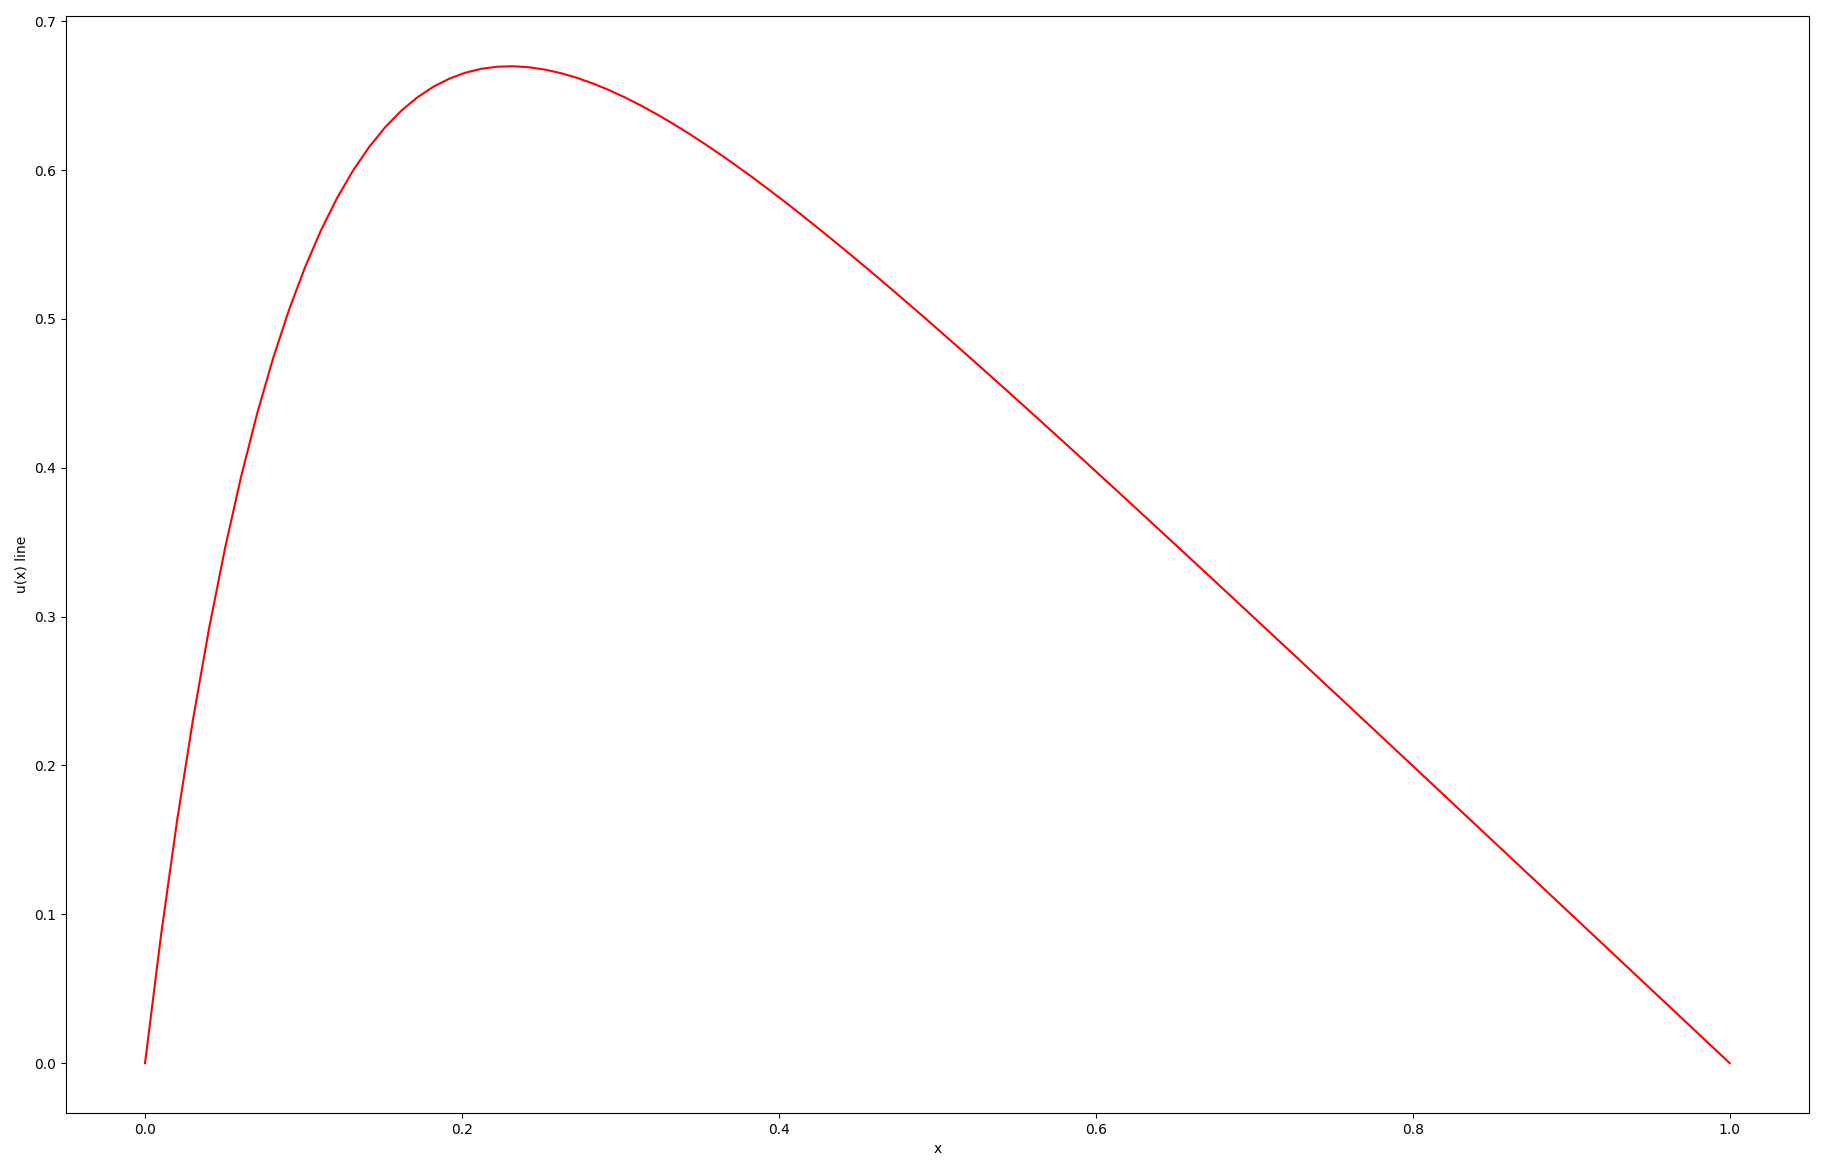
\includegraphics[width=1.0\linewidth]{figures/prob2.png}
  \caption{Graph for the analytical solution\label{fig:prob2}}
\end{figure}

\section{} % problem 3

We now want to solve the Poisson equation numerically, in order to achieve this
we will start by dicretizing the second derivative of $u(x)$ using the a Taylor
expansion, this gives:

\begin{equation}
    \frac{\dd{^{2}u(x)}}{\dd{x}^2} = \frac{u(x+h) - 2u(x) + u(x-h)}{h^2} + \mathcal{O}(h^2)
\end{equation}

with $h$ being the step size, which we consider constant. Now that we have our
expansion we can approximate $v_i(x) \approx u_i(x)$ giving us the approximation
of $\mathcal{O}(h^2)$ and the discretized Poisson equation:

\begin{align*}
     -\frac{v_{i+1} - 2v_i + v_{i-1}}{h^2} \approx f_i
\end{align*}

%continue proof reading here


\section{} % problem 4

As seen in Problem 3 we have come with a discretized version of our ODE with a
step h constant creating $n_{\text{step}} + 1$ discrete values of v and f. 
Here we have this relation between number of steps and number of unknowns that our matrix
equation has, $n = n_{\text{step}} - 1$ so $n + 1 = n_{\text{step}}$\\

We can remark that the Taylor expansion we used to define a discrete version of
the second derivative for a step i requires the previous and future step value
of our function v. Causing a problem for the boundaries values $v_0$ and 
$v_{n_{\text{step}}}$ since for the first case $v_0$ we do not have a previous step $v_{-1}$
and for $v_{n + 1}$, $v_{n + 2}$ is not defined as well. However we
may not be able to numerically compute the boundaries values of v but we are able to
calculate all the intermediates values. \\

In consequence, we will have the relations for all $v_i$ $i \in \{1, ..., n\}$:

\begin{align*}
    2v_1 - v_2 &= h^2f_1 + v_0 \\
    -v_1 + 2v_2 - v_3 &= h^2f_2 \\
    -v_2 + 2v_3 - v_4 &= h^2f_3 \\
    \vdots \\
    -v_{n-1} + 2v_{n} &= h^2f_{n} + v_{n + 1}   
\end{align*}

From this we can see that the left side of every equation is known because
$f(x)$ is given, h is a controlled parameter and $v_0$ and $v_{n + 1}$ are our
boundaries conditions hence we know their value. \\
From this we define $g_i = h^2f_i$ for $i \in \{ 2, ... , n\}$, $g_1 = h^2f_1 + v_0$, $g_{n} = h^2 f_{n} + v_{n + 1}$ and the column vector 


\begin{equation*}
    \vec{g}=\begin{bmatrix}
    g_1 \\
    g_2 \\
    \vdots \\
    g_{n}
\end{bmatrix}
\end{equation*}

For the right side, we define $\vec{v}$ a $1 \times n$ vector containing all
the approximated solution except for our two bondaries points which are known
and by defining $\mathbf{A}$ a $n \times n$ matrix

\begin{align}
\mathbf{A}\vec{v} = \begin{bmatrix}
                 2 & -1 & 0 & 0 & \dots & 0 \\
                 -1 & 2 & -1& 0 & \dots & 0\\
                 0 & -1 & 2 & -1 & \dots & 0\\
                 \vdots & \ddots &  \ddots & \ddots & \ddots & \vdots \\
                 0 & \ddots &  \ddots & -1 & 2 & -1 \\
                 0 & \dots &  \dots & 0 & 2 & -1
                 \end{bmatrix}
                 \begin{bmatrix}
                     v_1 \\
                     v_2 \\
                     v_3 \\
                     \vdots \\
                     v_{n - 1} \\
                     v_{n}
                 \end{bmatrix}
\end{align}
With these definitions, we have rewritten our system of discretized equations to
a matrix equation: $\mathbf{A}\vec{v} = \vec{g}$.




\section{} % problem 5

\subsection{a)}
if we define $\vec{v}^{*}$ the complete solution of length m and
$\mathbf{A}$ the matrix of size $n\times n $ define in a similar way as problem
4. In order to transform our system of equations we had to ignore the boundaries
conditions as they were ill-defined due to the discretization of the second
derivative. With that in mind, the complete solution must contain the boundaries
conditions so if we have m discrete values and a square matrix of size n without
two values, we have the following relation: $n = m-2$.

\subsection{b)}
In a) and problem 4 we established a matrix equation to solve $\vec{v}$ containing all points except for the boundary points so solving this matrix equation gives us all values of $v_i$ with $i \in \{1, \dots, n\}$.



\section{} % problem 6
\subsection{a)}
We have the matrix equation $\boldsymbol{A}\vec{v} = \vec{g}$ with
$\boldsymbol{A}$ being a general tridiagonal matrix. In order to solve this
equation we will proceed in two steps. The first one, known as forward
substitution consist in doing matrix operation to obtain an upper triangular
matrix and the last step, backwards substitution, which will give us our
approximation $\vec{v}$.
The algorithm works by transforming  $\boldsymbol{A}$ to the identity matrix,
modifying $\vec{g}$ along the way.In the end we see that the solution to
$\vec{v}$ will equal the modified $\vec{g}$. Now let's see in detail how we can
perform the algorithm. \\

We have: \[
\boldsymbol{A} = \begin{bmatrix}
                 b_1 & c_1 & 0 & 0 & \dots & 0 \\
                  a_2 & b_2 & c_2 & 0 & \dots & 0\\
                 0 & a_3 & b_3 & c_3 & \dots & 0\\
                 \vdots & \ddots &  \ddots & \ddots & \ddots & \vdots \\
                 0 & \ddots &  \ddots & a_{n-1} & b_{n-1} & c_{n-1} \\
                 0 & \dots &  \dots & 0 & a_{n} & b_{n}
                 \end{bmatrix}
\]
\\

We perform the operation: $R_2 \rightarrow R_2 - \frac{a_2}{b_1}R_1$ which
implies that the second row becomes
$R_2 = [0, b_2 - \frac{a_2}{b_1}c_1, 0, \dots, 0]$ and the second element of
$\vec{g}$ becomes $\Tilde{g_2} := g_2 - \frac{a_2}{b_1}c_1$. We define
$\Tilde{b_2}:= b_2 - \frac{a_2}{b_1}c_1$, $\Tilde{b_1}:= b_1$ and
$\Tilde{g_1} := g_1$. \\

We can see that performing the general operation:
$R_i = R_i - \frac{a_i}{\Tilde{b_{i-1}}}R_{i-1}$ for $i \in \{2, ..., n\}$ and
defining $\Tilde{b_i} := b_i -\frac{a_i}{\Tilde{b_{i-1}}}c_{i-1}$,
$\Tilde{g_i} := g_i - \frac{a_i}{\Tilde{b}_{i-1}}\Tilde{g}_{i-1}$ will lead us
to:

\[
                 \begin{bmatrix}
                 \Tilde{b_1} & c_1 & 0 & 0 & \dots & 0 \\
                  0 & \Tilde{b_2} & c_2 & 0 & \dots & 0\\
                 0 & 0 & \Tilde{b}_3 & c_3 & \dots & 0\\
                 \vdots & \vdots &  \vdots & \vdots & \vdots & \vdots \\
                 0 & \dots &  \dots & 0 & \Tilde{b}_{n-1} & c_{n-1} \\
                 0 & \dots &  \dots & 0 & 0 & \Tilde{b_{n}}
                 \end{bmatrix}
                \vec{v}
                =
                \begin{bmatrix}
                    \Tilde{g_1} \\
                    \Tilde{g_2} \\
                    \Tilde{g_3} \\
                    \vdots \\
                    \Tilde{g}_{n-1} \\
                    \Tilde{g_n} \\
                \end{bmatrix}
\]

The first step is now complete and we start the last step. First we observe that
all coefficient from $\vec{a}$, $\vec{b}$ and $\vec{c}$ is known, therefore we
can see that the last row yields the following relation:
$\Tilde{b}_n v_n = \Tilde{g}_n \Rightarrow v_n = \frac{\Tilde{g}_n}{\Tilde{b}_n}$
\\

By making the row operation $R_n \rightarrow \frac{R_n}{\Tilde{b}_n}$ we 'clear'
the nth row and we have found the first value of our numerical solution $v_n$.
Now that we know $v_n$ we can go back one rank to find the value of $v_{n-1}$
and we repeat the process in order to find $v_{n-2}$ until we find the last
value $v_1$. So we can generalize the row operation needed:

\begin{equation*}
    R_{n-1} \rightarrow \frac{R_{n-1} - c_{n-1}R_n}{\Tilde{b}_{n-1}}
\end{equation*}

which allows us to write an expression for $v_{n-1}$

\begin{equation*}
        v_{n-1} = \frac{\Tilde{g}_{n-1}-c_{n-1}v_n}{\Tilde{b}_{n-1}}
\end{equation*}

By repeating the operation enough time to find all values of $v_i$ giving us the
relation for $v_i$:

\begin{align*}
    v_n &= \frac{\Tilde{g}_n}{\Tilde{b}_n} \\
    v_i &= \frac{\Tilde{g}_i - c_i v_{i+1}}{\Tilde{b}_i} \quad i \in \{1, \dots, n-1\} 
\end{align*}


\subsection{b)}
To count the FLOPs for this algorithm we start by looking at how many FLOPs is
needed for the forwards substitution.
To start of we determine $\Tilde{b}_1$ as:

\begin{equation}
  \Tilde{b}_1 = b_1
  \label{eq_gen_algo_I}
\end{equation}

Then we proceed to do the following calculations for every $n \in \{2,\dots n\}$:

\begin{align}
	d &= \frac{a_i}{\Tilde{b}_{i-1}} \\
  \Tilde{b}_i &= b_i - d \cdot c_{i-1}
  \label{eq_gen_algo_II} \\
  \Tilde{g}_i &= g_i - d \cdot \Tilde{g}_{i-1}
  \label{eq_gen_algo_III}
\end{align}

the first line uses 1 FLOPs, and each of the lines below uses 2 FLOPs. They are repeated 
$(n-1)$ times.  Hence we have $2(n-1) + 2(n-1) + (n - 1) = 5(n-1)$ FLOPs for the Forward substitution.
 \\

For the backwards substitution we start off by calculating the last element of vector $v$.

\begin{equation}
  v_n = \frac{\Tilde{g}_n}{\Tilde{b}_n}
  \label{eq_gen_algo_IV}
\end{equation}

next we calculate the remaining elements of $v$ by:

\begin{equation}
  v_i = \frac{\Tilde{g}_i - c_iv_{i+1}}{\Tilde{b}_i} \quad i \in \{n-1, \dots, 1\}
  \label{eq_gen_algo_V}
\end{equation}

The first step in the backwards substitution contributes a single FLOP, the
remaining iterations yield $3(n-1)$ FLOPs to the total FLOP-count.

Thus the total number of FLOPs for the Thomas-algorithm is $8 \times (n-1) + 1 = 8n - 7$

\section{} % problem 7
\subsection{a)}
main.cpp calls the function  \verb|gen_thoman_alg | from \verb|src/utils.cpp| to solve the
matrix equation $\bold{A}\vec{v} = \vec{g}$, where $\bold{A}$ is a general tridiagonal matrix.
The solution is written to a file with name \verb|general_thomas_<N>.txt|, where N is the number of points.

We define the vectors \verb|a|, \verb|b|, \verb|c| , \verb|g| and \verb|v| with \verb|n| where the first three of these define the signature $(-1, 2, -1)$ of the three diagonals in our matrix. the \verb|g|-vector is initialized by \verb|g = h*h*f(x)|.

We explicitly force the boundary values at $v_{n + 1} = 0$ 
and $v_0 = 0$ and iterate over the inner points. The vectors 
$\Tilde{b}$ and $\Tilde{g}$ are defined as 
$b\_$ and $g\_$ respectively. 
We then implement the algorithm as defined in task 6. (In our program
 the variable $n_{\text{steps}}$ is the total number of points.)

\subsection{b)}
\begin{figure}[H]
  \centering
  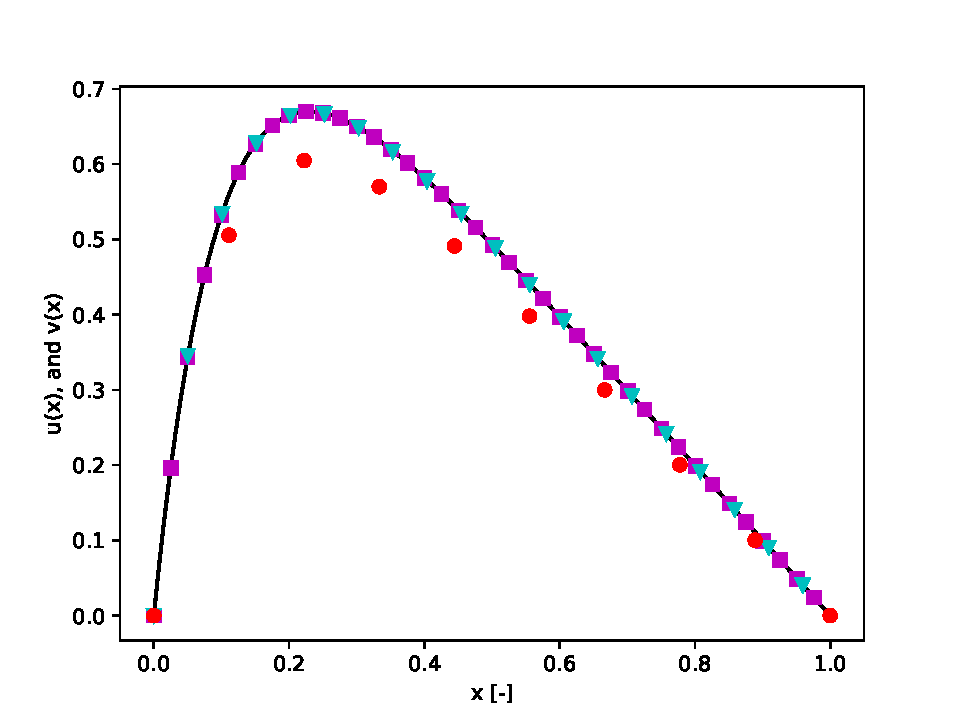
\includegraphics[width=1.0\linewidth]{figures/plot_7.pdf}
  \caption{Plot of numerical approximation and excact solution (black line) for different number of steps, red circle is $n_{\text{steps} } = 10$, cyan triangle is $n_{\text{steps} } = 100$, and magenta
    square is $n_{\text{steps} } = 1000$. We see a signinficant improvement in the accuracy when we increase from $10$ to $100$ steps. By eye we don't see a significant difference between $100$ and $1000$ steps.}
\label{fig_plot7}
\end{figure}

In \ref{fig_plot7} we can see the exact solution $u(x)$ and the numerical approximation $v_i$. By eye we can see a significant improvement when we increase the number of steps from $10$ to $100$, it is however
difficult to see a difference in accuracy between $100$ and $1000$ steps.


\section{} % problem 8
\subsection{a)}
\begin{figure}[H]
  \centering
  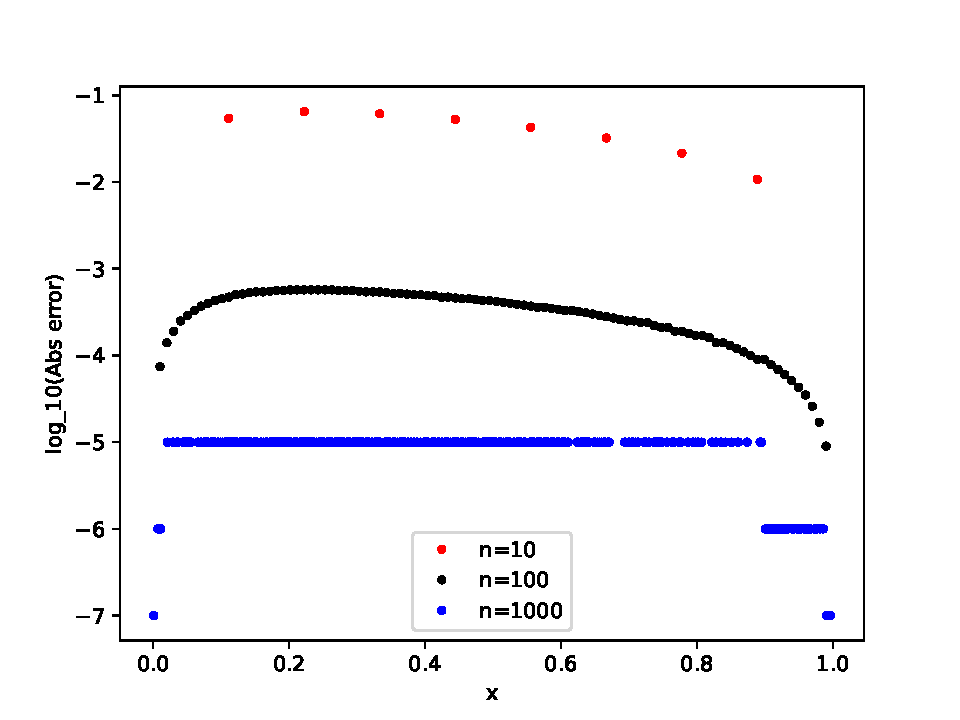
\includegraphics[width=1.0\linewidth]{figures/plot_8a.pdf}
  \caption{Plot of $\log_{10}{\Delta_i}$}
  \label{fig_plot8a}
\end{figure}


We make plots \ref{fig_plot8a} of the absolute error, $\Delta_i = \abs{u_i - v_i}$ in every inner point using
\verb|plot8.py|. We see that the errors are smaller closer to the boundaries for all.

\subsection{b)}
\begin{figure}[H]
  \centering
  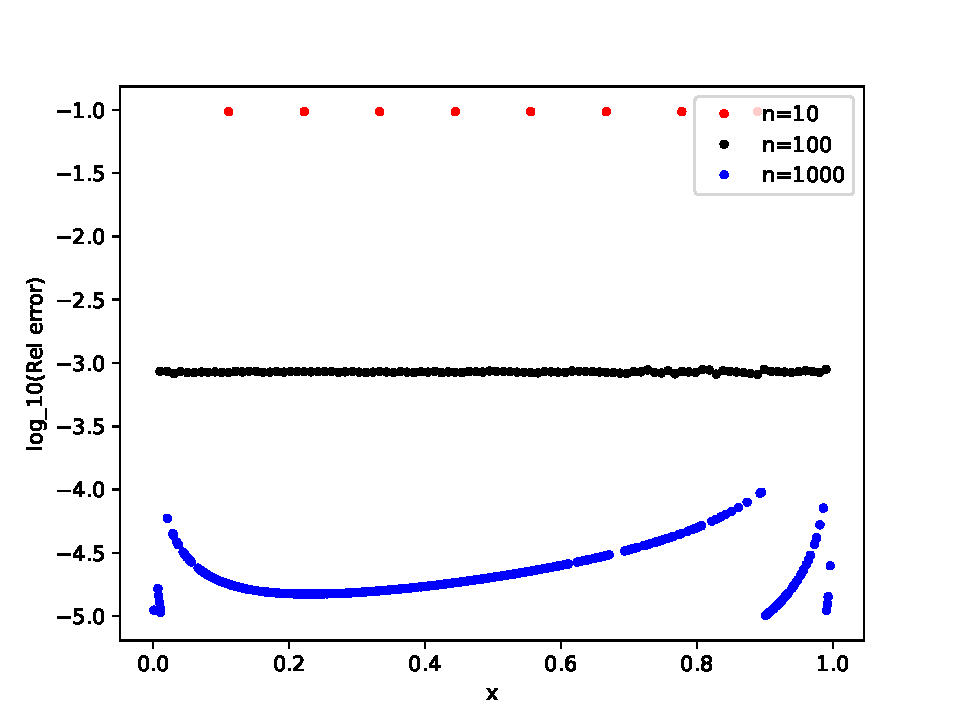
\includegraphics[width=1.0\linewidth]{figures/plot_8b.pdf}
  \caption{Plot of $\log_{10}{\varepsilon_i}$}
  \label{fig_plot8b}
\end{figure}

Plot \ref{fig_plot8b} shows the relative error for various number of points. The errors are reduced by two
orders of magnitude when we increase the number of points from $10$ to $100$. In this range our error
is of $\mathcal{O}(h^2)$, we see that the truncation error dominates. Near the boundaries we see that the
relative error increases for the smallest stepsize. This may be due to possible catastrophic cancellations
in \ref{eq_gen_algo_II},  \ref{eq_gen_algo_III}, or  \ref{eq_gen_algo_V}.
n
\subsection{c)}
 \begin{tabular}{ |c||c|}
 	\hline
 	\multicolumn{2}{|c|}{Maximum relative error for various number of steps.} \\
 	\hline
 	$n_{\text{steps}}$ & Max relative error \% \\
 	\hline
   10 & 9.7 \\
   100 & 0.089 \\
   $10^3$ & 0.10 \\
   $10^4$ & 0.009 \\
   $10^5$ & 0.004 \\
   $10^6$ & 0.010 \\
   $10^7$ & 0.010 \\
   \hline
\end{tabular}


The table above shows the maximum relative error for different step size. For the smallest number of points, i.e 10, we have the worst error close to 10$\%$ and as we increase the number of points we reduces the error as expected but we remark that around $10^5$ points, increasing the number of points actually augment the maximum relative error. We can explain this on the first thought, a contradicting result but as we have seen in class we have two types of errors, the mathematical error due to our approximation and the round-off error due to the computer limited memory. We have seen that reducing the 'distance' between our points would give us a better answer but it will start to increase the round-off error as our step size will get smaller and smaller we have higher chance of catastrophic cancellation. Hence we have to reduce the gap between our points but we have to take in account that doing so will increase the error associated with the computer's memory showing us that an optimal step size is not the smallest possible but an intermediate one minimizing both types of error.  

\section{} % problem 9

\subsection{a)}

In this case we have: $\vec{a}=\{-1, -1, \dots, -1\}$, $\vec{b}=\{2,2, \dots, 2\}$
and $\vec{c} = \{-1, -1, \dots, -1\}$.

So by using equation (8) and inserting the constant values for $a_i$ we get

\begin{align*}
	g_i = g_i + \frac{\Tilde{g}_{i - 1}}{\Tilde{b}_{i - 1}}
\end{align*}

And using the same trick but with the equation for $v_i$ and inserting for $c_i$ we get

\begin{align*}
	v_i = \frac{\Tilde{g}_i + v_{i + 1}}{\Tilde{b}_i}
\end{align*}

For $\Tilde{b}_i$ we use that since $b_i$ is constant we calculate the first few terms

\begin{align*}
	\Tilde{b}_1 &= 2 \\
	\Tilde{b}_2 &= \frac{3}{2}
	\Tilde{b}_3 &= \frac{4}{3}
\end{align*}

we can see that it makes this pattern for $`Tilde{b}_i = \frac{i + 1}{i}$. \\

\subsection{b)}

All of these three operations takes two FLOPs each time and is done $(n - 1)$ times. However
we still need to calculate $v_n = \frac{\Tilde{g_n}}{\Tilde{b_n}}$, so the total FLOPs of the special algorithm is 
$3 (n - 1) + 1 = 3n - 2$


\subsection{c)}

In the same way as problem 7.1 a), we use main.cpp. Howevere here it calls the function \verb|gen_thoman_alg | from \verb|src/utils.cpp| and makes this file \verb|special_thomas_<N>.txt|, where N is the number of points.

This code has the same structure as task 7 but with different algorithms for $\Tilde{b}_i$, $\Tilde{g}_i$ and $v_i$, also no $b_i$, $a_i$ and $c_i$ were defined.

\section{} % problem 10

In this question, we try to compare the execution time for both our algorithms with different step size. In order to compute the execution time we used the chrono function from the C++ library given in the project description. We run the program up to $10^6$ steps 5 times every time. It allowed us to compute the mean execution time and we use the standard deviation formula to calculate the error. The results are presented in the table underneath. 


\begin{tabular}{ |c||c|c|}
	\hline
	\multicolumn{3}{|c|}{Execution time between Thomas algorithm and The special algorithm} \\
	\hline
	Step size N & Thomas algorithm [s] &Special algorithm [s] \\
	\hline
	10     &  6.3960e-06$\pm$1.1729e-06   & 4.7944e-06$\pm$4.1929e-6	\\
	100    &  3.14726e-05$\pm$1.4968e-05& 1.34792e-05$\pm$3.6568e-05     \\
	$10^3$ &0.0002013$\pm$9.371e-05		 & 0.00010249$\pm$2.7006e-05\\
	$10^4$ &0.00163008$\pm$0.00037397        & 0.0013955$\pm$0.0003512 \\
	$10^5$ &  0.0135912$\pm$0.0021826      & 0.01068024$\pm$0.00043691 \\
	$10^6$ & 0.127284$\pm$0.00466895      & 0.109234$\pm$0.00438743 \\
	\hline
\end{tabular}

We can observe that the special algorithm is always a bit faster than the general one which is what we would expect with the FLOPs calculated in the previous exercises. However we can note that the time difference is minimal and we can explain it by the fact that both algorithm are of order $O(N)$ so both execution time scale linearly with N and the optimizations done on both code reduces the execution time but the differences between the two algorithm should not be due to the step size as it increases the execution time linearly for both code.

\end{document}
